\documentclass[twoside,11pt]{article}
\usepackage{amssymb,amsmath, amsfonts,latexsym,mathtext, array, graphicx, geometry, caption, subcaption, enumitem}
\geometry{margin=1.5cm}
\setlength{\parskip}{0.8ex plus 0.1ex minus 0.2ex}
\newcommand{\M}[1]{\boldsymbol{\mathbf{#1}}}
\newcommand{\V}{\M}
\newcommand{\Cal}{\mathcal}


\begin{document}
\newtheorem{thm1}{Theorem}
\newtheorem{def1}{Definition}


\title{Machine Learning 6.867 - Pset 2}

\maketitle
%!TEX root = pset2.tex

\section{Logistic Regression}\label{sec:lr}

\subsection{Implementation}
We implemented $L_2$-regularized logistic regression using gradient descent.

\subsection{Testing in data with $\lambda = 0$}
We test the logistic regression 

\begin{figure}[h!]
\centering
    \begin{subfigure}[b]{0.4\textwidth}
	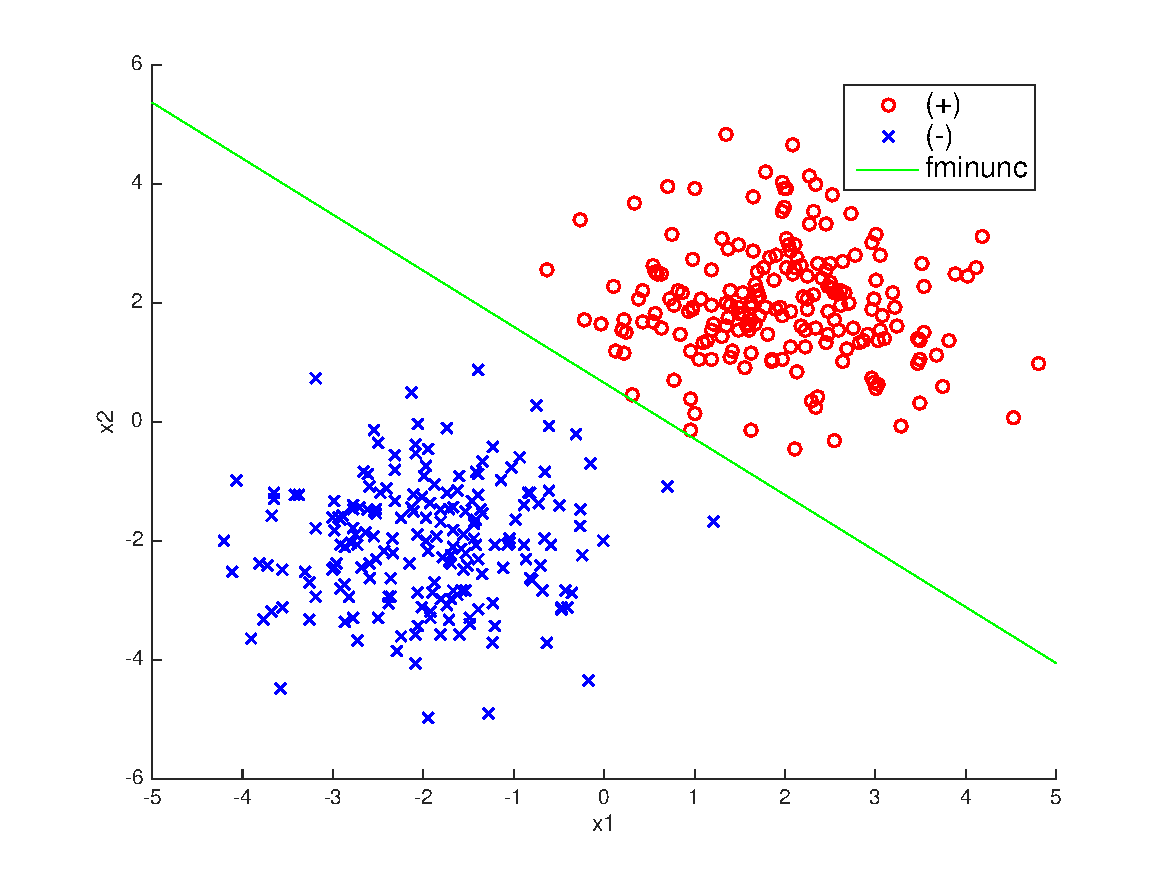
\includegraphics[scale=0.4]{hw2_11.pdf}
	\caption{Data with $\sigma = 1$}\label{fig:data_stdev1}
    \end{subfigure}
    \quad
    \begin{subfigure}[b]{0.4\textwidth}
	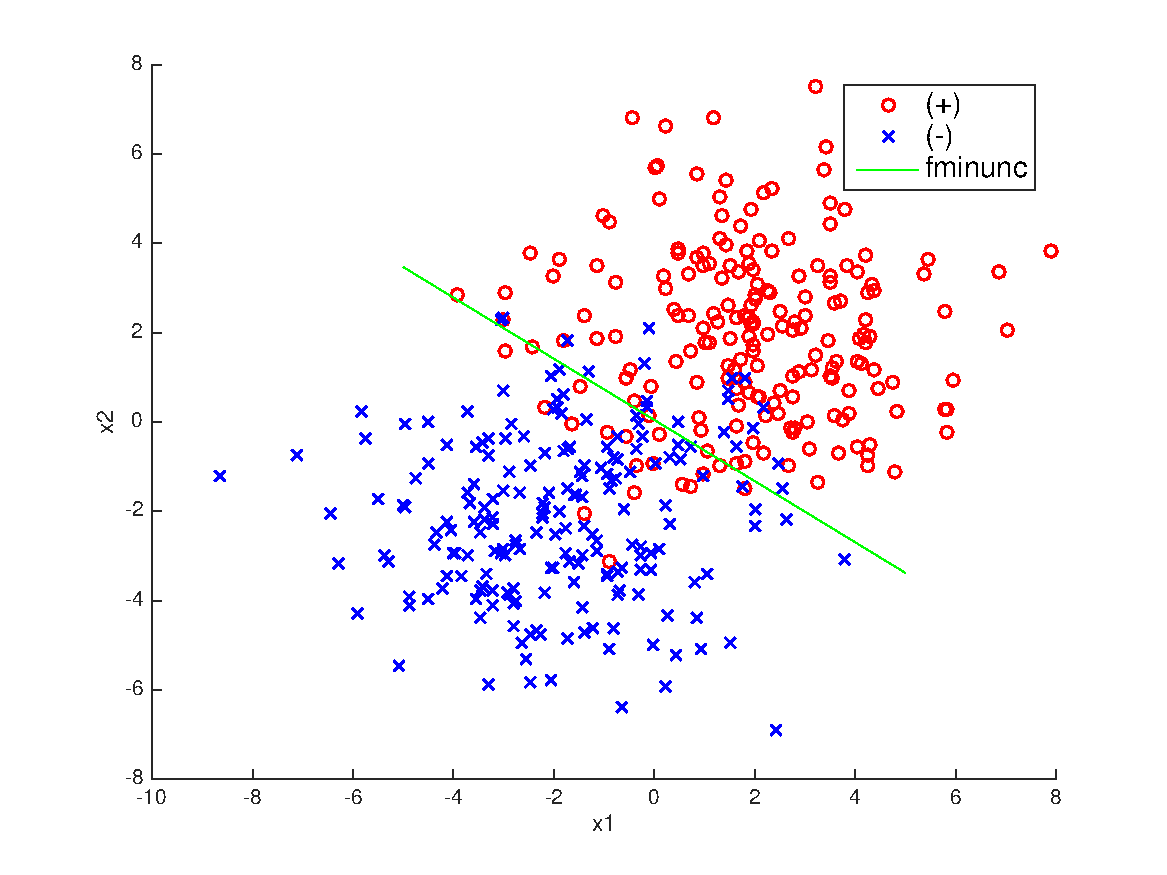
\includegraphics[scale=0.4]{hw2_12.pdf}
	\caption{CData with $\sigma = 2$}\label{fig:data_stdev2}
	\end{subfigure}
	
    \quad
    
    \begin{subfigure}[b]{0.4\textwidth}
	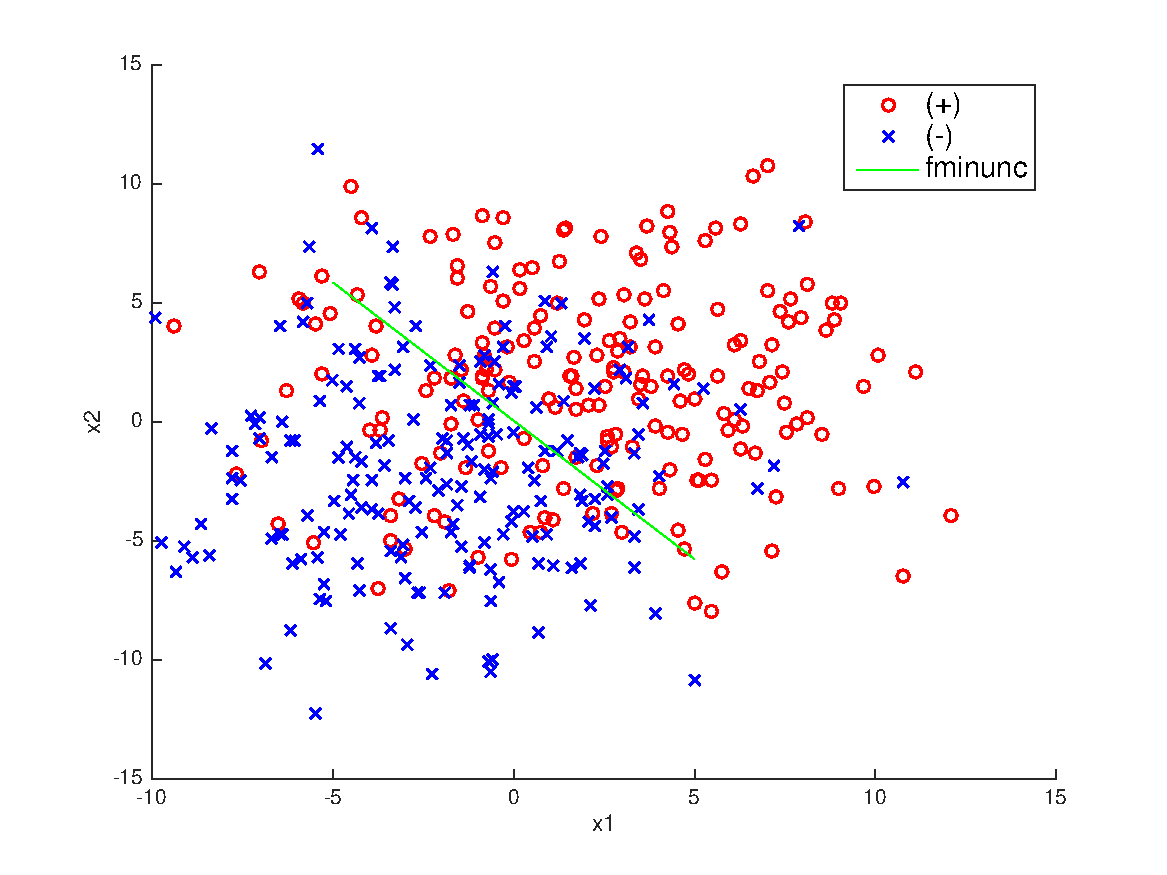
\includegraphics[scale=0.4]{hw2_13.pdf}
	\caption{Data with $\sigma = 4$}\label{fig:data_stdev4}
    \end{subfigure}  
    \quad
    \begin{subfigure}[b]{0.4\textwidth}
	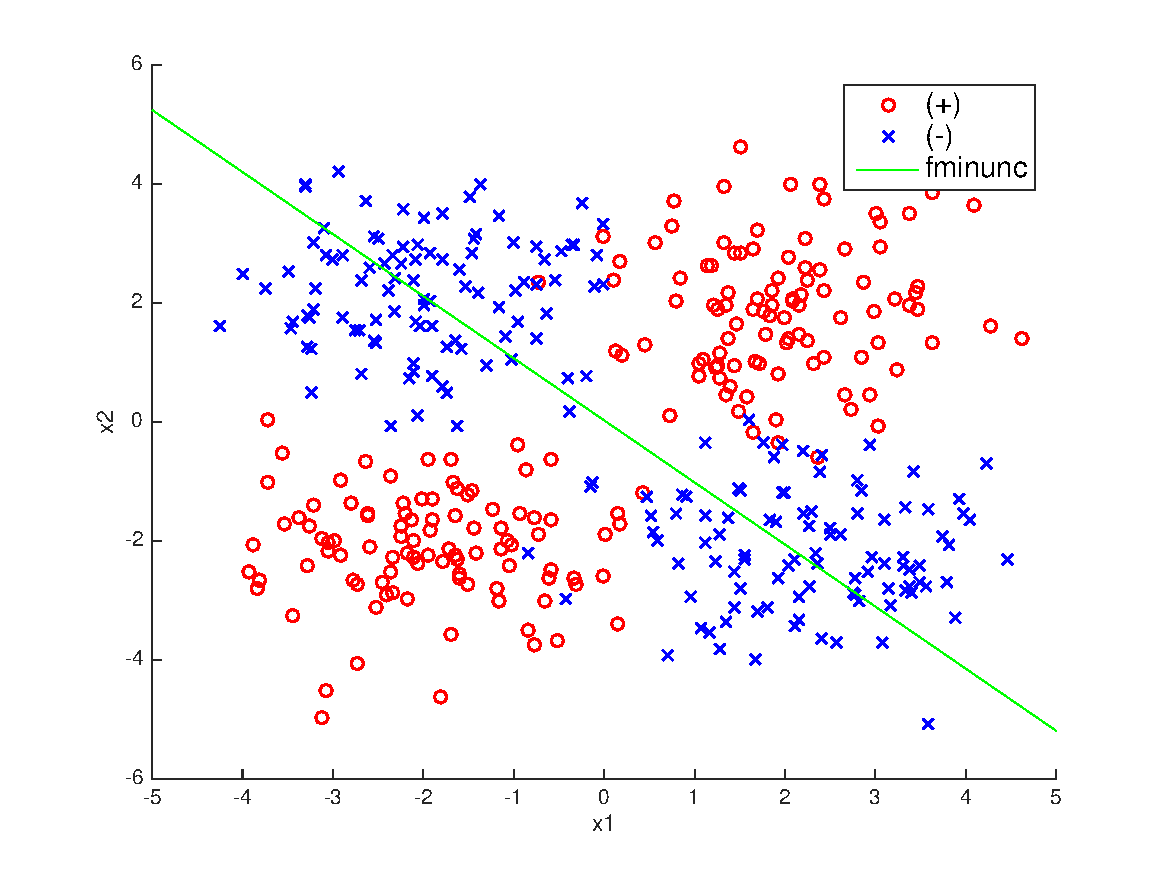
\includegraphics[scale=0.4]{hw2_14.pdf}
	\caption{Non-seperable data}\label{fig:data_nonsep}
    \end{subfigure}  
    \caption{}    
\end{figure}


%!TEX root = pset2.tex

\section{Support Vector Machine}\label{sec:svm}

Support Vector Machines are a popular classification method to construct linear or nonlinear decision boundaries
by solving a convex optimization problem.  There are two common forms of the optimization problem considered for SVM,
which we refer to as the primal and dual.  In this paper, we only consider the dual form, because it is computationally more tractable
for many problems, and this method has the ability to generalize to different choices of kernel.  The dual form of SVM for a general
kernel function $k: \mathcal{X} \times \mathcal{X} \rightarrow \mathbb{R}$ is as follows:

\begin{equation}
\label{eq:svm_dual}
\begin{array}{rll}
\underset{\alpha \in \mathbb{R}^n}{\max}~ & \sum\limits_{i = 1}^n \alpha_i 
- \frac{1}{2} \sum\limits_{i = 1}^n\sum\limits_{j = 1}^n \alpha_i \alpha_j y^{(i)} y^{(j)} k(x^{(i)}, x^{(j)}) \vspace{3pt}\\
\textup{s.t.}~ & 0 \leq \alpha_i \leq C,&~~~i=1,\ldots ,n, \vspace{3pt}\\
& \sum\limits_{i = 1}^n \alpha_i y^{(i)} = 0. & \\
\end{array}
\end{equation}

\subsection{Implementation}

First, we implemented the dual form of the SVM with a linear kernel, where $k$ is the usual dot product $k(x, z) = \langle x,z \rangle$ for all $x, z \in \mathcal{X}$. 
In MATLAB, we created a function with inputs: data $X \in \mathbb{R}^{n \times p}$, labels $Y \in \{-1,1\}$, and cost parameter $C \in \mathbb{R}^{+}$. 
Within the function, we use the quadratic solver \texttt{quadprog} to solve the SVM dual problem (\ref{eq:svm_dual}) with these parameters to find the optimal $\alpha$'s.
Since \texttt{quadprog} requires that the problem fit into a certain functional form, we reformulate the problem (\ref{eq:svm_dual}) as follows:

\begin{equation}
\label{eq:svm_dual2}
\begin{array}{rll}
-\underset{\alpha \in \mathbb{R}^n}{\min}~ & \frac{1}{2} \alpha^T H \alpha - \sum\limits_{i = 1}^n \alpha_i \vspace{3pt}\\
\textup{s.t.}~ & 0 \leq \alpha_i \leq C,&~~~i=1,\ldots ,n, \vspace{3pt}\\
& \sum\limits_{i = 1}^n \alpha_i y^{(i)} = 0, & \vspace{5pt}\\
\end{array}
\end{equation}
where:  $H \in \mathbb{R}^{n \times n}$ is a matrix with $(i,j)^{th}$ entry $H_{ij} = y^{(i)} y^{(j)} k(x^{(i)}, x^{(j)})$.  Given the optimal solution $\alpha \in \mathbb{R}^n$ for the SVM problem with a linear kernel, the chosen linear decision boundary $\theta^T x + \theta_0 = 0$ is given by:

\begin{equation}
\label{eq:svm_theta}
\theta = \sum\limits_{i = 1}^n \alpha_i y^{(i)} x^{(i)}
\end{equation}
\begin{equation}
\label{eq:svm_theta_0}
\theta_0 = \frac{1}{\mathcal{M}} \Big(\sum\limits_{j \in \mathcal{M}} \Big(y^{(j)} - \sum\limits_{i \in \mathcal{S}}\alpha_i y^{(i)} (x^{(j)})^T x^{(i)} \Big)\Big)
\end{equation}

The output of our linear SVM function is $[\theta, \theta_0]$.  We tested our function on the 2D example $X = \{(1,2),(2,2),(0,0),(-2,3)\}$, $Y = \{1,1,-1,-1\}$.  
For this problem, the objective function generated for problem (\ref{eq:svm_dual2}) is:

\begin{equation}
\label{eq:svm_objective1}
\frac{1}{2} \alpha^T H \alpha - \sum\limits_{i = 1}^4 \alpha_i,
\end{equation}
where:
\[
H = \begin{bmatrix}
     5   &  6  &   0  &  -4 \\
     6   &  8  &   0  &  -2 \\
     0   &  0  &   0  &   0 \\
    -4   & -2  &  0  &   13 \\
\end{bmatrix}
\]

The constraints are:
%
\begin{equation}
0 \leq \alpha_i \leq C,~~~i=1,\ldots ,4,
\end{equation}
\begin{equation}
\alpha_1 + \alpha_2 - \alpha_3 - \alpha_4 = 0.
\end{equation}

\subsection{Performance on datasets}

We tested our linear SVM function on the same 2D datasets from the previous section, with parameter $C = 1$.  

% TODO

\subsection{Kernel SVM}

We extended our SVM implementation in MATLAB to operate with more general kernels, taking the kernel function or kernel matrix as input.  

%TODO: continue
%!TEX root = pset2.tex

\section{Titanic Data}\label{sec:tinanic}

\subsection{Logistic Regression}
We use Logistic Regression classifier on the Titanic data to make predictions on survivor results. Before running the regression, we scale the features in two ways: 1) standardizing using mean and standard deviation by $(X_{j}^{(i)} - \mu(X_{j}))/\sigma(X_{j})$; 2) scale so each dimension is within the $[0, 1]$ range using min and max: $(X_{j}^{(i)} - \min{X_j})/(\max{X_j} - \min{X_j})$. We find the scaling constants in the training sets only, and use the same constants in the validation and testing sets. Note comparing the two scaling methods is simply for exploration purposes and we are not choosing one or the other in the model selection process.

With no regularization, we obtain a testing set accuracy of $77.78\%$ in both cases of scaling methods. To find the best $\lambda$, we use the cross validation technique. The validation set accuracy with respect to $\lambda$ is presented in Figure \ref{fig:3_LR_cv}. We therefore choose $\lambda = 10$ in standard-deviation-based scaling, and $\lambda = 0.1$ in range-based scaling. on the validation accuracy. The test set accuracy is then $75.13\%$ and $76.19\%$, respectively. Unfortunately neither is not as good as the non-regularized logistic regression. Furthermore, the way how one scales the features can also impact the accuracy.

\begin{figure}[hb]
\centering
	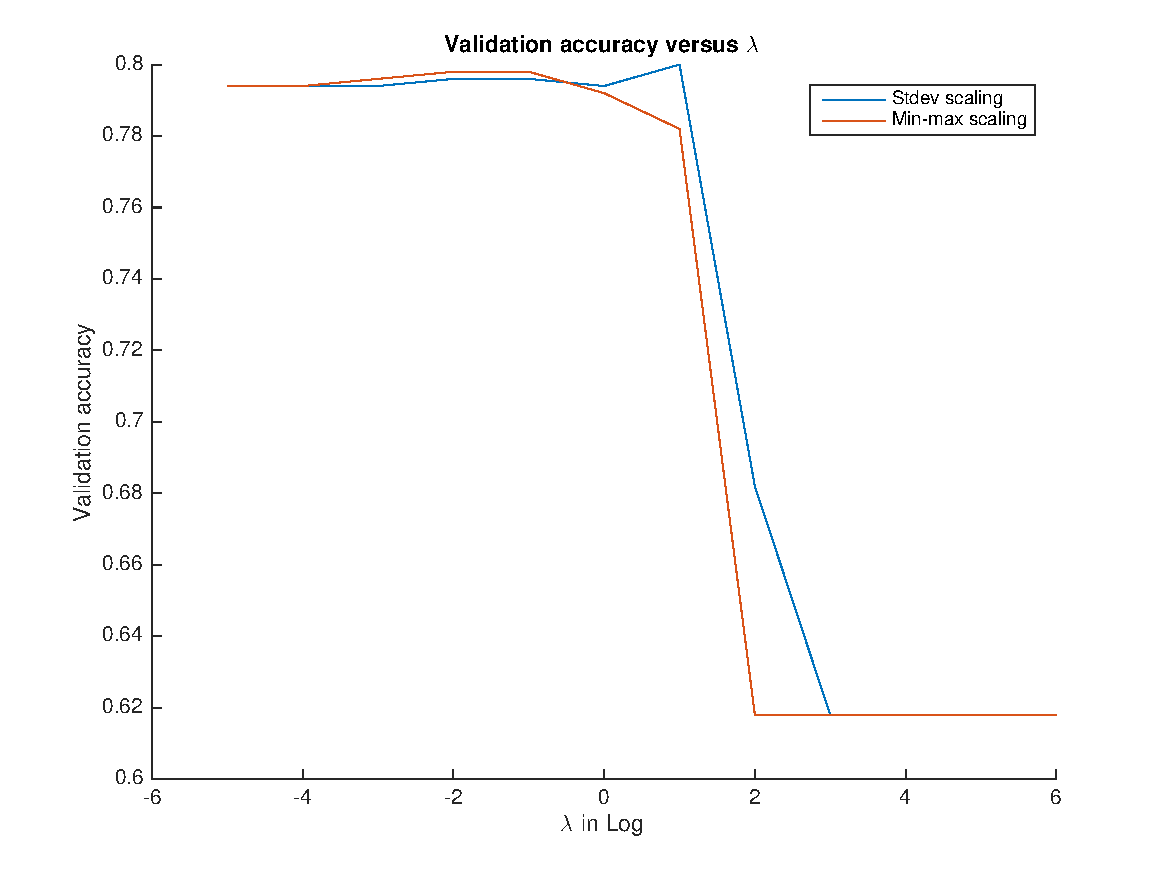
\includegraphics[scale=0.4]{hw2_3_cv.pdf}
	\caption{Tinanic Data, Cross validation error in logistic regression with respect to $\lambda$, under two different scaling methods.}\label{fig:3_LR_cv}
\end{figure}


\subsection{SVM}
TODO

\subsection{Comparison}
TODO compare LR and SVM

The estimated coefficients for logistic regression and SVM are presented in Table \ref{tab:titanic_coeff}. Since we do not have standard error and confidence interval information, we can only rely on the magnitude of the estimator (even if they are not statistically significant). 

We observe that being woman, higher class and higher fare are associated with higher likelihood of survival, whereas being 3rd class is strongly associated with death. 

\begin{table}[h!]
\centering
\caption{Estimated logistic regression coefficients in Titanic data, $\lambda = 10$}
\begin{tabular}{llr}
	\hline 
	Coefficient & Description & Logistic estimator \\
  \hline
  $w_0$  & Constant &-0.6289 \\
  $w_1$ 	& Passenger class 1 & 0.1680\\
  $w_2$ 	& Passenger class 2	  & 0.2013\\
  $w_3$  & Passenger class 3 & -0.3245\\
  $w_4$ 	 & Sex & 0.7795\\
  $w_5$ 	 & Age & -0.1417\\
  $w_6$ 	 & Num siblings/Spouses aboard & -0.0477 \\
  $w_7$ 	 & Num parents/children aboard & 0.1422\\
  $w_8$ 	 & Pasenger fare & 0.1533\\
  $w_9$ 	 & Port of embarkation = Southampton & -0.0955\\
  $w_{10}$  & Port of embarkation = Cherbourg & 0.1090\\
  $w_{11}$ & Port of embarkation = Queenstown	& 0.0393	\\
  \hline
\end{tabular}\label{tab:titanic_coeff}
\end{table}






\end{document}